% The solver-first chain vs. the decision-support loop.
%
% Single source for the diagram in
%   optimization-private/lecture-notes/lectures/optimization-for-decision-support.tex
% which \input's this file via \figsrc. Rendered to ../media/figures/decision-loop.{png,svg}
% by `make` so the website can show the same picture.
%
% Greyscale: the encoding is REDUNDANT by construction. The naive chain is
% dashed AND grey AND labelled "the solver-first picture"; the loop is solid
% AND black AND labelled. Either the line style or the text carries the
% contrast on its own, so nothing is lost on a mono laser printer.
%
% ⚠ DRAWN IN BLACK AND GREY, NOT BLUE -- a considered decision, not an
% oversight. scripts/check_greyscale.py runs on the RENDERED IMAGE, and a thin
% coloured stroke antialiases into a family of intermediate tones. The blue
% version of this drawing (the tints it carried while it lived inline in the
% lecture: NavyBlue at !70, !75, !8 and !85) reported FIVE data colours and
% FOUR failing pairs -- all of them edge pixels no reader would ever perceive
% as series. Black and grey blend only into greys, which the checker
% recognises as monochrome and passes outright. All three pre-existing tenants
% of this directory -- pendulum, farmer-crop-allocation, reactor-selection --
% are black line art and all three PASS, so this follows the house precedent
% rather than inventing a rule. Nothing is lost: the contrast was already
% carried by solid-vs-dashed and by the two written captions.
%
% NOTE this is a real change from what the lecture printed before the move.
% It had never been through the greyscale gate, because no TikZ written inside
% a .tex is reachable by it. Moving it here is what exposed the failure.

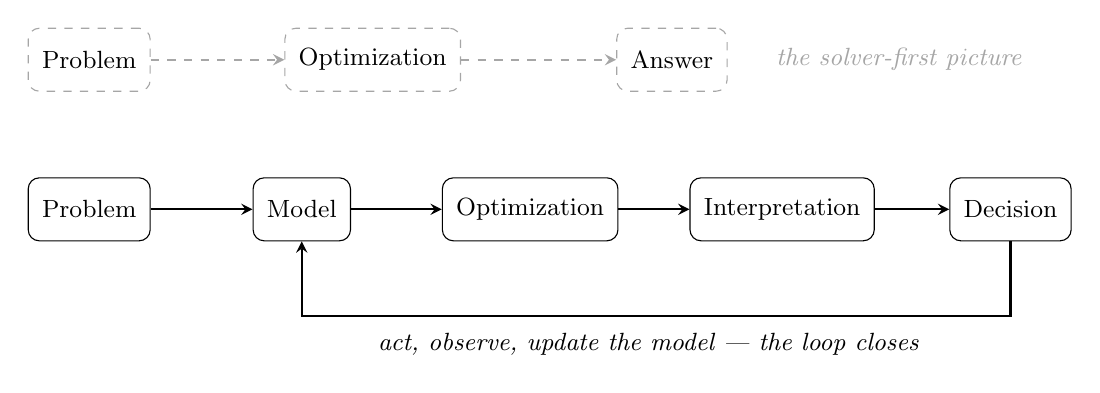
\begin{tikzpicture}[>=stealth,
    stage/.style={draw=black, fill=white, rounded corners,
                  minimum height=8mm, inner xsep=5pt, font=\small, align=center},
    naive/.style={draw=gray!70, fill=white, dashed, rounded corners,
                  minimum height=8mm, inner xsep=5pt, font=\small, align=center},
    flow/.style={->, thick, draw=black},
    nflow/.style={->, thick, dashed, draw=gray!70}]

  % ---- the naive chain: DASHED and GREY (redundant with the label below)
  \node[naive] (nA) at (0.0,1.9) {Problem};
  \node[naive] (nB) at (3.6,1.9) {Optimization};
  \node[naive] (nC) at (7.4,1.9) {Answer};
  \draw[nflow] (nA) -- (nB);
  \draw[nflow] (nB) -- (nC);
  \node[gray!70, font=\small\itshape, anchor=west] at (8.6,1.9)
    {the solver-first picture};

  % ---- the loop: SOLID (redundant with the label)
  \node[stage] (A) at (0.0,0.0)  {Problem};
  \node[stage] (B) at (2.7,0.0)  {Model};
  \node[stage] (C) at (5.6,0.0)  {Optimization};
  \node[stage] (D) at (8.8,0.0)  {Interpretation};
  \node[stage] (E) at (11.7,0.0) {Decision};
  \draw[flow] (A) -- (B);
  \draw[flow] (B) -- (C);
  \draw[flow] (C) -- (D);
  \draw[flow] (D) -- (E);

  % ---- the return path: this is what makes it a loop rather than a chain
  \draw[flow] (E.south) -- ++(0,-0.95) -| (B.south);
  \node[black, font=\small\itshape] at (7.1,-1.72)
    {act, observe, update the model --- the loop closes};
\end{tikzpicture}
